% Artículo autocontenido. Compilar dos veces con pdflatex.
\documentclass[11pt,a4paper]{article}
\usepackage[utf8]{inputenc}
\usepackage[T1]{fontenc}
\usepackage{lmodern,microtype}
\IfFileExists{spanish.ldf}{\usepackage[spanish,es-tabla,es-nodecimaldot,es-noshorthands]{babel}
\ifdefined\spanishplainpercent\spanishplainpercent\fi}{\usepackage{babel}\babelprovide[import,main]{spanish}}
\usepackage[margin=26mm]{geometry}
\usepackage{amsmath,amssymb,mathtools,amsthm,booktabs,tabularx,array,enumitem,xcolor,pgfplots}
\pgfplotsset{compat=1.16}
\usepackage[colorlinks=true,linkcolor=black,citecolor=teal,urlcolor=teal]{hyperref}
\definecolor{verde}{HTML}{18655C}
\setlength{\emergencystretch}{1.4em}
\newtheorem{teorema}{Teorema}
\newcommand{\R}{\mathbb R}
\newcommand{\E}{\mathbb E}
\newcommand{\T}{^{\mathsf T}}
\newcommand{\eps}{\varepsilon}
\newcommand{\nrm}[1]{\lVert #1\rVert}
\newcommand{\cO}{\mathcal O}
\newcommand{\pN}{p_{\mathrm N}}
\newcommand{\pS}{p_{\mathrm S}}
\newcommand{\HS}{\widetilde H}
\newcommand{\lS}{\widetilde\lambda}
\DeclareMathOperator{\diag}{diag}
\DeclareMathOperator{\col}{col}
\DeclareMathOperator{\nnz}{nnz}
\newcommand{\tema}[1]{\smallskip\par\textbf{#1}\enspace\ignorespaces}
\title{Newton Sketch: aproximación aleatoria de la curvatura y convergencia}
\author{Diego Alejandro Arévalo Arias\\[2pt]\small Álgebra Lineal Numérica y Optimización Numérica}
\date{Noviembre de 2026}
\begin{document}
\renewcommand{\abstractname}{Resumen}\renewcommand{\proofname}{Demostración}
\renewcommand{\refname}{Referencias}\renewcommand{\tablename}{Tabla}
\maketitle
\begin{abstract}
En problemas con muchas más observaciones que variables, formar el hessiano puede costar más que resolver el sistema de Newton. Newton Sketch comprime un factor rectangular de la curvatura y conserva el gradiente exacto. Estudiamos el algoritmo con tamaño de proyección fijo, mostramos cuatro construcciones sobre los mismos datos y demostramos una cota de convergencia lineal-cuadrática en el decremento para funciones autoconcordantes. En una regresión logística con 5000 observaciones, 100 variables y un sketch de 600 filas, el muestreo uniforme y CountSketch alcanzaron una tolerancia relativa de $10^{-4}$ en $7.43$ y $7.53$ ms, frente a $18.37$ ms de Newton exacto en la serie de la presentación. Los tres necesitaron cuatro iteraciones medianas. El coste de construir el factor comprimido explica por qué proyecciones de igual tamaño pueden producir tiempos distintos.
\end{abstract}

\section{Introducción}
En mínimos cuadrados y en regresión logística, cada observación aporta al hessiano una matriz de rango uno. Cuando hay $n$ observaciones y $d$ variables con $n\gg d$, se pueden emplear más operaciones en sumar esos $n$ aportes que en resolver el sistema de $d$ incógnitas. La pregunta es cuánta información sobre la curvatura necesita un modelo cuadrático para proponer una buena dirección.

Pilanci y Wainwright~\cite{PW17} plantean formar la matriz de Gram de una proyección aleatoria de las filas. La dimensión de los parámetros se conserva. El gradiente se calcula con todas las observaciones y, por tanto, un punto estacionario satisface la condición de optimalidad del objetivo original. El tamaño $m$ se elige antes de cada corrida. Los coeficientes aleatorios se renuevan en cada iteración.

La sección~\ref{sec:conceptos} relaciona el modelo de Newton con la autoconcordancia y el encaje de subespacios. La sección~\ref{sec:ns} construye el método, ilustra el papel de la búsqueda lineal y presenta la demostración. En la sección~\ref{sec:exp} la comparación se hace por tiempo hasta alcanzar una misma precisión certificada.

\section{Conceptos generales}\label{sec:conceptos}
\subsection{Modelo cuadrático y geometría local}
Sean $g=\nabla f(x)$ y $H=\nabla^2 f(x)\succ0$. El paso exacto minimiza el modelo
\begin{equation}
 q_x(p)=f(x)+g\T p+\tfrac12p\T Hp,\qquad H\pN=-g.\label{eq:modelo}
\end{equation}
El producto $g\T p$ es la pendiente inicial a lo largo de $p$. La forma $p\T Hp$ mide la curvatura en esa dirección. El hessiano define una norma local, su dual y el decremento de Newton,
\begin{equation}
 \nrm h_x=\sqrt{h\T Hh},\quad \nrm v_{x,*}=\sqrt{v\T H^{-1}v},\quad
 \lambda(x)=\nrm g_{x,*}=\nrm{\pN}_x.\label{eq:decremento}
\end{equation}
El modelo predice una disminución $\lambda(x)^2/2$. Para una cuadrática estrictamente convexa el modelo coincide con el objetivo y un paso completo alcanza el mínimo.

En una suma $f(x)=\sum_i\phi_i(a_i\T x)$ de pérdidas convexas dos veces diferenciables, $H=A\T DA=B\T B$, con $D_{ii}=\phi_i''(a_i\T x)$ y $B=D^{1/2}A$. Se forma $B$ al escalar cada fila de $A$. En mínimos cuadrados $D=I$. En regresión logística los pesos dependen de $x$. Cuando $H=B\T B$, la longitud local de un desplazamiento es precisamente $\nrm{Bp}_2$.

\subsection{Autoconcordancia en una y varias dimensiones}
Una función convexa $\varphi\in C^3(I)$ sobre un intervalo abierto es autoconcordante estándar si
\[
 |\varphi'''(s)|\le2\varphi''(s)^{3/2},\qquad s\in I .
\]
Donde $\varphi''>0$, esto equivale a $|(\varphi''^{-1/2})'|\le1$. La escala de longitud que determina la curvatura varía a una velocidad acotada. Para $\varphi(s)=-\log s$ en $s>0$, las derivadas segunda y tercera son $s^{-2}$ y $-2s^{-3}$ y se alcanza la igualdad. Para una cuadrática convexa la tercera derivada se anula. La exponencial, en cambio, tiene cociente $|\varphi'''|/(\varphi'')^{3/2}=e^{-s/2}$, que crece sin cota cuando $s\to-\infty$.

En un dominio abierto y convexo de $\R^d$, una función convexa $f\in C^3$ es autoconcordante estándar si cada restricción $t\mapsto f(x+th)$ lo es en su intervalo de definición. En derivadas direccionales,
\[
 |D^3 f(x)[h,h,h]|\le 2\bigl(h\T H(x)h\bigr)^{3/2}\quad\text{para todo }x,h .
\]
\tema{Ejemplo en el ortante positivo.}
Para $f(x)=-\sum_{i=1}^d\log x_i$, $H=\diag(x_i^{-2})$. Si $u_i=h_i/x_i$, las derivadas direccionales segunda y tercera son $\sum_i u_i^2$ y $-2\sum_i u_i^3$. Como $|\sum_i u_i^3|\le(\sum_i u_i^2)^{3/2}$ se verifica la condición. En $x=(1,2)$, los desplazamientos de norma local menor que uno forman la elipse $h_1^2+h_2^2/4<1$.

\tema{Ejemplo matricial.}
Para $F(X)=-\log\det X$ con $X=X\T\succ0$ y $U=U\T$, sean $\theta_j$ los autovalores de $X^{-1/2}UX^{-1/2}$. El incremento a lo largo de $X+tU$ es $-\sum_j\log(1+t\theta_j)$. Las derivadas de órdenes dos y tres en cero son $\sum_j\theta_j^2$ y $-2\sum_j\theta_j^3$. La misma desigualdad del ortante prueba la autoconcordancia. También toda cuadrática convexa en varias variables cumple la condición.

\tema{Consecuencias para Newton.}
Para $f$ cerrada, autoconcordante estándar y de hessiano definido positivo en su dominio abierto, el elipsoide abierto de Dikin $\{x+h:\nrm h_x<1\}$ está contenido en el dominio. Si $r=\nrm h_x<1$ se cumplen~\cite[sec.~9.6]{BV}
\begin{align}
 (1-r)^2H(x)&\preceq H(x+h)\preceq(1-r)^{-2}H(x),\label{eq:hesssc}\\
 f(x+h)&\le f(x)+g\T h+\omega_*(r),\qquad \omega_*(r)=-r-\log(1-r).\label{eq:valsc}
\end{align}
Aquí $M\preceq N$ significa $v\T Mv\le v\T Nv$ para todo $v$. Con el paso exacto amortiguado $\pN/(1+\lambda)$ se obtiene una disminución de al menos $\lambda-\log(1+\lambda)$. Cuando $\lambda<1$, el paso exacto completo satisface $\lambda(x+\pN)\le[\lambda/(1-\lambda)]^2$. La cota muestra la convergencia cuadrática local en una escala que incorpora la curvatura de cada dirección.

\subsection{Johnson--Lindenstrauss y encajes de subespacios}
Para $N$ puntos fijados, el lema de Johnson y Lindenstrauss~\cite{JL84} permite conservar todas las distancias al cuadrado dentro de factores $1\pm\eps$ en dimensión de orden $\eps^{-2}\log N$. Newton elige la dirección después de sortear $S$. Se necesita controlar simultáneamente los infinitos vectores $Bv$, que pertenecen a un subespacio de dimensión $r=\operatorname{rango}(B)$. La condición pertinente es
\begin{equation}
 (1-\eps)\nrm{Bv}_2^2\le\nrm{SBv}_2^2\le(1+\eps)\nrm{Bv}_2^2
 \quad\text{para todo }v\in\R^d.\label{eq:encaje}
\end{equation}
En forma de orden espectral, esto equivale a
\begin{equation}
 (1-\eps)B\T B\preceq B\T S\T SB\preceq(1+\eps)B\T B.\label{eq:loewner}
\end{equation}
Si $U$ tiene columnas ortonormales que generan $\col(B)$, la misma condición es $\nrm{U\T S\T SU-I}_2\le\eps$. La media $\E[S\T S]=I$ garantiza conservación en promedio, mientras que el encaje impone un control de cada dirección en la realización usada. Para un subespacio fijo, una matriz gaussiana normalizada logra este control con probabilidad al menos $1-\delta$ si $m\ge c\eps^{-2}(r+\log(1/\delta))$, con $c$ universal~\cite{MT20}.


\subsection{Ejemplos numéricos de las cuatro proyecciones}\label{sec:ejemplos}
Usamos la matriz y los pesos del ejemplo de Pluto. Los sorteos que siguen se eligen para verificar los productos a mano. El cuaderno genera los suyos con semilla 2026.
\[
 A=\begin{pmatrix}1&0\\0&1\\1&1\\-1&2\\2&-1\end{pmatrix},\quad
 w=(1,1/2,1,1/2,1)\T,\quad
 B=\diag(w)A=\begin{pmatrix}1&0\\0&1/2\\1&1\\-1/2&1\\2&-1\end{pmatrix}.
\]
En los cuatro casos $S$ mide $3\times5$ y $C=SB$ mide $3\times2$.

\tema{Gaussiano.} Se toma $S=G/\sqrt m$ con entradas de $G$ normales estándar independientes. Con coeficientes gaussianos redondeados a dos decimales, y usando esos valores redondeados para efectuar el producto, se obtiene
\[
 S=\frac1{\sqrt3}\begin{pmatrix}-.79&.24&-1.90&1.40&.64\\-.29&-.31&.30&-.27&-.23\\.72&.51&-.06&-.09&.16\end{pmatrix},\quad
 C=\frac1{\sqrt3}\begin{pmatrix}-2.110&-1.020\\-.315&.105\\1.025&-.055\end{pmatrix}.
\]
Cada fila de salida mezcla las cinco observaciones. El producto denso cuesta $\cO(mnd)$. Generar los coeficientes por paneles reduce el almacenamiento temporal.

\tema{CountSketch.} La columna $i$ tiene una entrada $s_i\in\{-1,1\}$ en la posición $h(i)$ escogida uniformemente. Cada fila de $B$ aporta a un único destino. Con los signos y destinos de las diapositivas,
\[
 S=\begin{pmatrix}0&-1&0&1&0\\1&0&0&0&-1\\0&0&1&0&0\end{pmatrix},\qquad
 C=\begin{pmatrix}-1/2&1/2\\-1&1\\1&1\end{pmatrix}.
\]
La primera fila es $b_4\T-b_2\T$. Las colisiones mezclan observaciones que pueden tener mucha influencia. La aplicación cuesta $\cO(\nnz(B)+md)$ con salida densa y una cota suficiente clásica de tamaño en el peor caso es $\cO(r^2/(\delta\eps^2))$ para una entrada por columna.

\tema{Muestreo uniforme de filas (RowSampling).} Para los índices $(2,5,2)$ escogidos con reemplazo,
\[
 S=\sqrt{5/3}\begin{pmatrix}0&1&0&0&0\\0&0&0&0&1\\0&1&0&0&0\end{pmatrix},\qquad
 C=\sqrt{5/3}\begin{pmatrix}0&1/2\\2&-1\\0&1/2\end{pmatrix}.
\]
El factor $\sqrt{n/m}$ garantiza la normalización en media. Leer $m$ filas con acceso directo cuesta $\cO(md)$. Un subespacio cuya información se concentra en pocas filas puede quedar mal representado. Para medir esa concentración se usan las puntuaciones de palanca $\ell_i=\nrm{e_i\T U}_2^2$. Si se muestrea con probabilidades $\pi_i=\ell_i/r$, cada fila seleccionada se pondera por $1/\sqrt{m\pi_i}$. El experimento usa la versión uniforme.

\tema{Transformada de Hadamard aleatorizada submuestreada (SRHT).} Se extiende $B$ con tres filas nulas hasta $N=8$, se cambian signos con una diagonal $D_\pm$, se aplica la matriz ortogonal de Walsh--Hadamard $W_N$ y se eligen tres filas mediante $R_m$. Así $C=\sqrt{N/m}\,R_mW_ND_\pm B_{\rm ext}$. Con signos $(+,-,+,-,+)$ sobre las filas originales, orden de Sylvester y coordenadas de salida $(1,3,6)$,
\[
 S=\frac1{\sqrt3}\begin{pmatrix}1&-1&1&-1&1\\1&-1&-1&1&1\\1&1&1&1&-1\end{pmatrix},\qquad
 C=\frac1{\sqrt3}\begin{pmatrix}9/2&-3/2\\3/2&-3/2\\-1/2&7/2\end{pmatrix}.
\]
Aquí $S$ es el operador efectivo sobre las cinco filas. La mezcla distribuye la energía antes del submuestreo. La transformada completa por sumas y restas requiere $\cO(Nd\log N)$ operaciones~\cite{MT20,PW17}.

\section{Newton Sketch}\label{sec:ns}
\subsection{Modelo y búsqueda lineal}
En $x_k$ escribimos $g_k=\nabla f(x_k)$ y $H_k=B_k\T B_k+P_k$, donde $P_k\succeq0$ es una parte de la curvatura fácil de formar, por ejemplo $P_k=\mu I$. Se usa un nuevo $S_k\in\R^{m\times n}$ en cada iteración con $m$ fijo. Si $C_k=S_kB_k$, el modelo comprimido y su hessiano son
\begin{equation}
 \widetilde q_k(p)= f(x_k)+g_k\T p+\tfrac12\nrm{C_kp}_2^2+\tfrac12p\T P_kp,\qquad
 \HS_k=C_k\T C_k+P_k.\label{eq:parcial}
\end{equation}
Con $\HS_k\succ0$ el paso satisface $\HS_k\pS=-g_k$, y $g_k\T\pS=-\pS\T\HS_k\pS<0$ siempre que $g_k\ne0$. El decremento aproximado es $\lS_k=\sqrt{-g_k\T\pS}$.

\begin{enumerate}
\item Evaluar la función, el gradiente completo y los pesos que determinan $B_k$. Verificar el criterio de parada.
\item Sortear $S_k$, formar $C_k$ y construir $\HS_k$. Resolver el sistema para $\pS$ mediante una factorización. Para $P_k=\mu I$ con $\mu>0$, el sistema es definido positivo aun si $C_k$ pierde rango.
\item Partir de $\alpha=1$ y multiplicar por $\beta\in(0,1)$ hasta que el candidato pertenezca al dominio y $f(x_k+\alpha\pS)\le f(x_k)+a\alpha g_k\T\pS$, con $0<a<1/2$.
\item Aceptar $x_{k+1}=x_k+\alpha\pS$ y repetir hasta alcanzar la tolerancia o el límite prescrito.
\end{enumerate}
El coste denso de formar el producto de Gram disminuye de $\cO(nd^2)$ a $\cO(md^2)$ una vez disponible $C_k$. Hay que sumar el coste de la proyección, del gradiente, de la búsqueda lineal y del sistema de orden $d$, cuya factorización cuesta $\cO(d^3)$.

\subsection{Un paso con CountSketch}
La presentación considera mínimos cuadrados con el mismo $S$ de CountSketch del ejemplo anterior y nuevos datos,
\[
 A=\begin{pmatrix}1&0\\0&1\\1&1\\2&0\\0&2\end{pmatrix},\quad
 b=(2,1,0,2,0)\T,\quad SA=\begin{pmatrix}2&-1\\1&-2\\1&1\end{pmatrix}.
\]
Para $f(x)=\nrm{Ax-b}_2^2/2$ desde $x_0=0$, se tiene $g_0=(-6,-1)\T$ y
\[
 H=\begin{pmatrix}6&1\\1&6\end{pmatrix},\quad
 \HS=\begin{pmatrix}6&-3\\-3&6\end{pmatrix},\quad
 \pN=(1,0)\T,\quad \pS=(13/9,8/9)\T.
\]
El paso exacto alcanza $x^\star=(1,0)\T$ y $f^\star=3/2$. El comprimido tiene pendiente $-86/9$. Con $\alpha=1$ la distancia euclídea al óptimo baja de $1$ a $0.994$, mientras que la brecha sube de $3$ a $3.358$. La función mide el error como $(x-x^\star)\T H(x-x^\star)/2$. Armijo con $a=0.1$ y $\beta=1/2$ rechaza el paso completo y acepta $\alpha=1/2$, con brecha $0.701$.

Si se mantiene esta realización de $S$ fija en la cuadrática, los valores propios de $\HS^{-1}H$ son $5/9$ y $7/3$. Con el paso unitario un modo del error se multiplica por $-4/3$. Con el paso constante $9/13$, los dos factores son $\pm8/13$. Esto explica la diferencia entre las dos trayectorias de las diapositivas.

\subsection{Demostración de la convergencia}
La formulación siguiente explicita el argumento autoconcordante de Pilanci y Wainwright~\cite[secs.~4.1 y 6.2]{PW17}. Las constantes se eligen para hacer transparente el control del retroceso y del paso completo.
\begin{teorema}\label{th:ns}
Sea $f$ cerrada, convexa y autoconcordante estándar, con mínimo alcanzado y hessiano definido positivo en su dominio abierto. Supóngase que, en el paso $k$, el sketch es un encaje de $\col(B_k)$ con distorsión $0\le\eps\le1/8$. Sean $0<a\le1/4$ y $0<\beta<1$ los parámetros de Armijo. Si $\lambda_k>1/8$, el retroceso ideal obtiene un descenso de al menos $7a\beta/1152$. Si $\lambda_k\le1/8$, se acepta el paso completo y
\begin{equation}
 \lambda_{k+1}\le\tfrac43\eps\lambda_k+\tfrac{16}{9}\lambda_k^2
                 \le\tfrac7{18}\lambda_k.\label{eq:lq}
\end{equation}
Si el encaje tiene probabilidad condicional al menos $1-\delta_k$ por paso, el resultado vale conjuntamente en los primeros $K$ pasos con probabilidad al menos $1-\sum_{k<K}\delta_k$.
\end{teorema}
\begin{proof}
\textit{Del encaje al residuo.}
Omitimos los subíndices y escribimos $p=\pS$, $\lambda=\nrm g_{x,*}$ y $r=\nrm p_x$. Al sumar la parte $P\succeq0$ a la aproximación de los datos se obtiene $(1-\eps)H\preceq\HS\preceq(1+\eps)H$. Definamos $M=H^{-1/2}\HS H^{-1/2}$ y $z=H^{-1/2}g$. El espectro de $M$ está en $[1-\eps,1+\eps]$, $H^{1/2}p=-M^{-1}z$ y $H^{1/2}\pN=-z$. Por tanto,
\begin{align}
 r&\le\lambda/(1-\eps), &
 \nrm{g+Hp}_{x,*}=\nrm{p-\pN}_x&\le\eps\lambda/(1-\eps),\label{eq:res}\\
 \frac{\lambda^2}{1+\eps}\le\lS^2&=z\T M^{-1}z\le\frac{\lambda^2}{1-\eps},&
 -g\T p=p\T\HS p&\ge(1-\eps)r^2 .\label{eq:dec}
\end{align}
La primera cota de error usa $\nrm{I-M^{-1}}_2\le\eps/(1-\eps)$. Para $g=0$ ya se ha alcanzado el mínimo.

\textit{Aceptación de Armijo.}
Para $0\le u<1$, se tiene $\omega_*(u)=\int_0^u t/(1-t)\,dt\le u^2/[2(1-u)]$. Por~\eqref{eq:valsc} y~\eqref{eq:dec}, para $\alpha r<1$ basta que
\[
 \frac{\alpha}{2(1-\alpha r)}\le(1-a)(1-\eps).
\]
Toda $\alpha\le s=1/[2(1+r)]$ cumple la condición, pues el lado izquierdo es a lo sumo $1/2$ y el derecho al menos $21/32$. La búsqueda acepta entonces $\alpha\ge\beta s$. Resulta
\[
 f(x)-f(x+\alpha p)\ge a\alpha\lS^2
 \ge\frac{a\beta\lambda^2}{2(1+\eps)(1+\lambda/(1-\eps))}.
\]
Este cociente crece con $\lambda$ y decrece con $\eps$. Sustituir ambos por $1/8$ prueba la cota para la primera fase. Cuando $\lambda\le1/8$ se tiene $r\le1/7$ y el paso completo cumple la condición, pues $1/[2(1-r)]\le7/12<21/32$.

\textit{Variación del gradiente.}
Sea $x^+=x+p$ en la región de pasos completos. El resto de Taylor es
\[
 R=\nabla f(x+p)-g-Hp=\int_0^1[H(x+tp)-H]p\,dt.
\]
Por~\eqref{eq:hesssc}, todos los autovalores de $H^{-1/2}H(x+tp)H^{-1/2}$ están entre $(1-tr)^2$ y $(1-tr)^{-2}$. Su distancia a uno es a lo sumo $(1-tr)^{-2}-1$, de modo que
\[
 \nrm R_{x,*}\le r\int_0^1 [(1-tr)^{-2}-1]\,dt=\frac{r^2}{1-r}.
\]
La comparación de hessianos en $t=1$ también da $\nrm v_{x+p,*}\le\nrm v_{x,*}/(1-r)$. Aplicada a $g+Hp+R$ junto con~\eqref{eq:res}, implica
\[
 \lambda(x+p)\le\frac{\eps\lambda}{(1-\eps)(1-r)}
                       +\frac{r^2}{(1-r)^2}.
\]
Como $r\le\lambda/(1-\eps)$ y $[(1-\eps)(1-r)]^{-1}\le4/3$, se sigue~\eqref{eq:lq}. Finalmente, condicionando a la historia previa a cada sorteo, $B_k$ está fijado. La cota de la unión sobre los fallos de encaje da la probabilidad anunciada.
\end{proof}

\tema{Intuición de la demostración.}
El paso exacto cancela el gradiente del modelo, $g+H\pN=0$. El paso comprimido cancela el de su propio modelo y deja un residuo de tamaño proporcional a $\eps\lambda$ en el modelo exacto. Al movernos al nuevo punto, el hessiano también cambia. La autoconcordancia limita la contribución acumulada de ese cambio a un término de orden $\lambda^2$. El gradiente que encuentra la siguiente iteración es la suma de ambos errores. Con curvatura exacta desaparece el término lineal. Con distorsión fija, este término puede dominar al acercarse al mínimo.

Sobre una trayectoria de encajes válidos, hay a lo sumo $1152(f(x_0)-f^\star)/(7a\beta)$ pasos antes de entrar en $\lambda\le1/8$. Esta región es invariante por~\eqref{eq:lq}, y $f(x)-f^\star\le\omega_*(\lambda(x))$ cuando $\lambda<1$~\cite{BV}. La contracción del decremento conduce así a una contracción geométrica de la cota de brecha en la fase local.


\section{Pruebas numéricas}\label{sec:exp}
\subsection{Modelo, instancia y criterio experimental}
En el experimento del proyecto, cada observación consta de una fila $a_i\T\in\R^{1\times d}$ y una etiqueta $y_i\in\{-1,1\}$. La pérdida penaliza los márgenes $y_i a_i\T x$ pequeños o negativos. El objetivo usa la \emph{suma} de pérdidas y regulariza las $d$ coordenadas,
\begin{equation}
 f(x)=\sum_{i=1}^n\log\!\left(1+\exp(-y_i a_i\T x)\right)
          +\frac{\mu}{2}\nrm{x}_2^2 . \label{eq:logistica}
\end{equation}
Con $p_i=\sigma(y_i a_i\T x)$ y $\sigma(t)=(1+e^{-t})^{-1}$, se forman los residuos $r_i=-y_i(1-p_i)$ y los pesos $D_{ii}=p_i(1-p_i)$. Las cantidades del algoritmo son
\begin{align*}
 g &=A\T r+\mu x, & B&=D^{1/2}A,\\
 H &=B\T B+\mu I, & \HS&=(SB)\T(SB)+\mu I .
\end{align*}
Una observación con margen cercano a cero tiene $p_i\simeq1/2$ y aporta el peso máximo $1/4$. Una con $p_i$ cercano a cero o a uno aporta poca curvatura. Una observación clasificada con mucha confianza en el sentido equivocado puede, por tanto, pesar poco en el hessiano y seguir aportando mucho al gradiente. Esta distinción ayuda a entender por qué el método calcula $g$ con todos los datos. En $x_0=0$, $B=A/2$. Luego los pesos se actualizan en cada paso.

\tema{Instancia del proyecto.}
Se fijaron $n=5000$, $d=100$, $\mu=0.5$ y la semilla $2026$. Se obtuvo una matriz ortogonal $Q$ por QR de una gaussiana cuadrada y se construyó $A=G\diag(1,1/2,\ldots,1/d)Q\T$, con $G$ gaussiana estándar independiente. La energía media de $A$ en la dirección $Qe_j$ decrece como $j^{-2}$. Para $u\sim\mathcal N(0,I_d)$ se formó $z=3Au/\operatorname{sd}(Au)$, donde $\operatorname{sd}$ es la desviación estándar muestral. Cada $y_i$ tomó el valor $1$ con probabilidad $\sigma(z_i)$. El óptimo empírico depende de las etiquetas y de la regularización.

Como $0\preceq D\preceq I/4$, se tiene $\mu I\preceq H\preceq(\mu+\nrm A_2^2/4)I$ y el objetivo tiene minimizador único. La cota inferior $\mu$ permite certificar la precisión alcanzada independientemente de la proyección. Este será el criterio común para cronometrar los cinco métodos.

\tema{Relación con la teoría local.}
Para $R=\max_i\nrm{a_i}_2$ se cumple $|D^3 f(x)[h,h,h]|\le (R/\sqrt\mu)\nrm h_x^3$. Con $R>0$, multiplicar el objetivo por $R^2/(4\mu)$ basta para obtener la normalización autoconcordante estándar. Este reescalamiento conserva el minimizador y la dirección de Newton. Los tiempos y las brechas que siguen corresponden a la escala original de~\eqref{eq:logistica}.

\tema{Qué significa alcanzar la misma precisión.}
Para una función $\mu$-fuertemente convexa, $f(x)-f^\star\le\nrm{\nabla f(x)}_2^2/(2\mu)$. Una resolución previa con Newton proporciona $x_{\rm ref}$. El óptimo queda entre $F_{\rm inf}=f(x_{\rm ref})-\nrm{\nabla f(x_{\rm ref})}_2^2/(2\mu)$ y $f(x_{\rm ref})$. En esta instancia $f(x_0)=3465.735903$, $F_{\rm inf}=2001.201730198640$ y la anchura del intervalo es aproximadamente $2.41\cdot10^{-10}$. Cada corrida se detiene en el primer iterado con
\begin{equation}
 \widehat\rho_k=\frac{f(x_k)-F_{\rm inf}}{f(x_0)-F_{\rm inf}}\le\tau,\qquad \tau=10^{-4}.\label{eq:target}
\end{equation}
Como $F_{\rm inf}\le f^\star$, esto implica $f(x_k)\le\tau f(x_0)+(1-\tau)f^\star$. La brecha real queda por debajo de una diezmilésima de la inicial. El umbral es $f(x_k)\le2001.348184$ (redondeado). El cuaderno exige además que la incertidumbre de la referencia sea a lo sumo el $1\,\%$ de $\tau(f(x_0)-F_{\rm inf})$.

\tema{Protocolo y procedencia.}
La presentación aporta la primera serie de mediciones y el informe del proyecto registra una segunda serie con el protocolo del cuaderno de Julia. Esta última se midió en Julia 1.11.7, con aritmética \texttt{Float64}, sobre un AMD EPYC 9V74 con un hilo de Julia y uno de OpenBLAS. La construcción de los datos, la referencia y el calentamiento se hicieron fuera del cronometraje. En siete rondas se barajó el orden de ejecución y se usaron semillas de proyección 2027 a 2033 sobre los mismos datos. Se emplearon Armijo con $a=0.1$ y $\beta=1/2$, un mínimo de paso de $2^{-40}$ y un máximo de 100 iteraciones. El tiempo total cuenta preparación y resolución, incluida la búsqueda lineal. Los MiB miden bytes acumulados asignados por Julia durante la corrida. Se publicó la mediana cuando las siete corridas alcanzaron la meta.

\subsection{Tiempo, memoria y brecha por iteración}
La tabla~\ref{tab:main} compara los métodos con $m=600=6d$. En la presentación, RowSampling tardó $7.43$ ms y CountSketch $7.53$ ms frente a $18.37$ ms de Newton exacto, aceleraciones de $2.47\times$ y $2.44\times$. En la segunda serie alcanzaron el mismo umbral en $2.34$ y $3.34$ ms frente a $8.37$ ms. Los tiempos de cada método deben compararse con la referencia de la misma serie.
\begin{table}[htbp]\centering\small
\caption{Tiempo mediano hasta $\tau=10^{-4}$ y memoria asignada. Los cinco métodos necesitaron cuatro pasos medianos. La segunda serie incluye siete éxitos por método.}\label{tab:main}
\begin{tabular}{@{}lrr rrr@{}}\toprule
&\multicolumn{2}{c}{Presentación}&\multicolumn{3}{c}{Segunda serie}\\
\cmidrule(lr){2-3}\cmidrule(l){4-6}
Método & ms & Asignación & ms $[Q_1,Q_3]$ & MiB & Aceleración\\ \midrule
Newton exacto & 18.37 & 4.1 MiB & 8.37 $[8.09,8.49]$ & 4.09 & $1.00\times$\\
Gaussiano & 127.82 & 8.7 MiB & 81.56 $[80.17,83.57]$ & 10.06 & $0.10\times$\\
CountSketch & 7.53 & 796 KiB & 3.34 $[3.27,3.38]$ & 0.81 & $2.51\times$\\
RowSampling & 7.43 & 716 KiB & 2.34 $[2.22,2.36]$ & 0.73 & $3.57\times$\\
SRHT & 18.32 & 1.1 MiB & 12.07 $[11.82,12.72]$ & 0.89 & $0.69\times$\\
\bottomrule\end{tabular}
\end{table}

El factor $C$ conserva el $12\,\%$ de las entradas de $B$, pues $m/n=600/5000$. Esta cuenta no incluye el espacio de trabajo ni la generación de los coeficientes. RowSampling accede a las filas seleccionadas y CountSketch las acumula en un único recorrido. El gaussiano denso usa más tiempo y memoria asignada en ambas series, pese a tener el mismo tamaño de salida. La SRHT completa hasta 8192 filas antes de la transformada.

La figura~\ref{fig:tray} muestra por qué llegar al mismo umbral puede dar brechas finales distintas. En el tercer paso, incluso Newton exacto supera todavía el umbral ($1.27\cdot10^{-4}$). En el cuarto llega a $2.41\cdot10^{-8}$, mientras que CountSketch y RowSampling llegan a $3.70\cdot10^{-5}$ y $5.66\cdot10^{-5}$, respectivamente. Una de las siete corridas gaussianas necesitó un quinto paso.
\begin{figure}[htbp]\centering
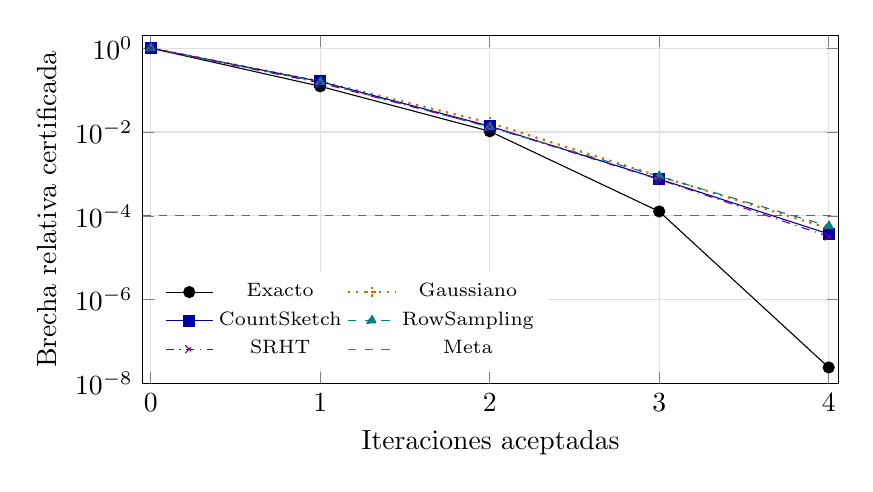
\begin{tikzpicture}
\begin{semilogyaxis}[width=.86\linewidth,height=6cm,xmin=-.05,xmax=4.06,ymin=1e-8,ymax=2,
xtick={0,1,2,3,4},ytick={1,1e-2,1e-4,1e-6,1e-8},xlabel={Iteraciones aceptadas},
ylabel={Brecha relativa certificada},grid=major,grid style={black!12},
legend style={at={(.02,.04)},anchor=south west,draw=none,font=\scriptsize},legend columns=2]
\addplot[black,mark=*] coordinates {(0,1)(1,.123)(2,.0104)(3,.000127)(4,2.41e-8)};\addlegendentry{Exacto}
\addplot[orange!85!black,dotted,thick,mark=+] coordinates {(0,1)(1,.161)(2,.0166)(3,.000878)(4,5.03e-5)};\addlegendentry{Gaussiano}
\addplot[blue!65!black,mark=square*] coordinates {(0,1)(1,.160)(2,.0138)(3,.000755)(4,3.70e-5)};\addlegendentry{CountSketch}
\addplot[teal,dashed,mark=triangle*] coordinates {(0,1)(1,.155)(2,.0130)(3,.000872)(4,5.66e-5)};\addlegendentry{RowSampling}
\addplot[violet,dashdotted,mark=x] coordinates {(0,1)(1,.148)(2,.0134)(3,.000737)(4,3.21e-5)};\addlegendentry{SRHT}
\addplot[black!60,dashed] coordinates {(-.05,1e-4)(4.06,1e-4)};\addlegendentry{Meta}
\end{semilogyaxis}\end{tikzpicture}
\caption{Brecha mediana sobre siete trayectorias, con $m=600$. La escala vertical es logarítmica.}\label{fig:tray}
\end{figure}

\subsection{Efecto del tamaño del sketch}
El barrido de la tabla~\ref{tab:barrido} mantiene fijos los datos y la tolerancia. Cada valor de $m/d$ define corridas completas en las que se vuelve a sortear $S_k$ en cada paso. Newton exacto tomó $8.37$ ms y cuatro iteraciones en la segunda serie.
\begin{table}[htbp]\centering\small
\caption{Tiempo mediano en milisegundos y mediana de pasos $k$ para siete corridas exitosas por configuración.}\label{tab:barrido}
\begin{tabular}{@{}rr rr rr rr rr@{}}\toprule
& &\multicolumn{2}{c}{Gaussiano}&\multicolumn{2}{c}{CountSketch}&
\multicolumn{2}{c}{RowSampling}&\multicolumn{2}{c}{SRHT}\\
\cmidrule(lr){3-4}\cmidrule(lr){5-6}\cmidrule(lr){7-8}\cmidrule(l){9-10}
$m/d$ & $m$ & ms & $k$ & ms & $k$ & ms & $k$ & ms & $k$\\ \midrule
1 & 100 & 42.94 & 10 & 8.26 & 11 & 3.82 & 9 & 28.23 & 10 \\
1.5 & 150 & 56.01 & 10 & 6.88 & 10 & 4.19 & 12 & 28.52 & 10 \\
2 & 200 & 50.70 & 7 & 4.93 & 7 & 3.41 & 9 & 20.39 & 7 \\
3 & 300 & 53.11 & 5 & 3.90 & 5 & 2.47 & 6 & 14.71 & 5 \\
4 & 400 & 58.08 & 4 & 3.84 & 5 & 2.31 & 5 & 14.63 & 5 \\
5 & 500 & 68.87 & 4 & 3.63 & 4 & 2.44 & 5 & 11.96 & 4 \\
6 & 600 & 81.56 & 4 & 3.34 & 4 & 2.34 & 4 & 12.07 & 4 \\
7 & 700 & 94.88 & 4 & 3.54 & 4 & 2.52 & 4 & 12.68 & 4 \\
8 & 800 & 105.61 & 4 & 3.67 & 4 & 2.59 & 4 & 12.21 & 4 \\
9 & 900 & 121.89 & 4 & 3.78 & 4 & 2.84 & 4 & 12.46 & 4 \\
10 & 1000 & 133.22 & 4 & 3.93 & 4 & 2.95 & 4 & 12.42 & 4 \\
\bottomrule
\end{tabular}
\end{table}

Con $m=100$, CountSketch necesitó once pasos y tardó $8.26$ ms. Con $m=600$ necesitó cuatro y tardó $3.34$ ms. Al pasar a $m=1000$ mantuvo los cuatro pasos y el tiempo subió a $3.93$ ms. La menor mediana de RowSampling apareció en $m=400$ ($2.31$ ms), incluso con un paso más que en $m=600$. Estos son mínimos observados en esta instancia.

\subsection{Distorsión espectral y coste del gaussiano}
En $x_0=0$, $m=600$ y con la semilla 2027, se calcularon los valores propios generalizados extremos de las matrices de Gram y del hessiano regularizado. Para este último, el cociente direccional es
\[
 \frac{v\T\HS v}{v\T Hv}=\frac{\nrm{Cv}_2^2+\mu\nrm v_2^2}{\nrm{Bv}_2^2+\mu\nrm v_2^2}.
\]
\begin{table}[htbp]\centering\small
\caption{Extremos de curvatura relativa en $x_0$ para una realización de cada proyección.}\label{tab:espectro}
\begin{tabular}{@{}lrrrr@{}}\toprule
& \multicolumn{2}{c}{Solo datos $(C\T C,B\T B)$}
& \multicolumn{2}{c}{Con $\mu I$ $(\HS,H)$}\\
\cmidrule(lr){2-3}\cmidrule(l){4-5}
Método & Mínimo & Máximo & Mínimo & Máximo\\ \midrule
Gaussiano & 0.369 & 1.947 & 0.592 & 1.572\\
CountSketch & 0.341 & 1.863 & 0.570 & 1.551\\
RowSampling & 0.360 & 2.063 & 0.567 & 1.636\\
SRHT & 0.376 & 1.878 & 0.596 & 1.555\\ \bottomrule
\end{tabular}
\end{table}

La regularización acerca los cocientes a uno. Por ejemplo, con CountSketch se observó una distorsión regularizada de $\max(1-0.570,1.551-1)=0.551$. La hipótesis $\eps\le1/8$ del teorema~\ref{th:ns} es suficiente y uniforme para todas las direcciones. Una corrida concreta puede progresar con mayor distorsión porque la dirección viene determinada por su gradiente y el paso se comprueba con Armijo.

La tercera prueba del cuaderno compara la generación de una nueva proyección gaussiana en cada iteración con reutilizar una sola matriz o un banco cíclico de cuatro. Para $m=600$, cada matriz en \texttt{Float64} ocupa $8mn$ bytes, unos $22.89$ MiB. Las dos estrategias que reutilizan coeficientes cambian la hipótesis de independencia del análisis. La comparación mide el trabajo que se ahorra al precalcularlos.
\begin{table}[htbp]\centering\small
\caption{Comparación gaussiana en la segunda serie. Los tiempos son medianas por columna.}\label{tab:banco}
\begin{tabular}{@{}lrrrrr@{}}\toprule
Estrategia & Preparación (ms) & Resolución (ms) & Total (ms) & Pasos & Banco (MiB)\\ \midrule
Nueva & 0.001 & 81.56 & 81.56 & 4 & 0.00\\
Una fija & 9.85 & 70.72 & 79.84 & 5 & 22.89\\
Cuatro cíclicas & 48.09 & 57.64 & 121.69 & 4 & 91.55\\ \bottomrule
\end{tabular}
\end{table}

La preparación elevó el tiempo total del banco de cuatro a $121.69$ ms, aunque la resolución sola duró $57.64$ ms. El total de cada corrida suma sus dos fases antes de tomar la mediana. En una serie instrumentada, generar coeficientes nuevos consumió en promedio $27.918$ ms por corrida, ponderar las filas $0.875$ ms y multiplicar los paneles $49.773$ ms. Aun con coeficientes almacenados, los pesos de la regresión cambian y exigen un nuevo producto en cada paso.

\section{Conclusiones}
El encaje del espacio columna vincula una operación sobre las filas con una garantía sobre el siguiente iterado. El término $\eps\lambda_k$ cuantifica lo que deja sin cancelar la dirección aproximada. El término $\lambda_k^2$ cuantifica cuánto cambia la curvatura al desplazarse al nuevo punto. La búsqueda lineal controla el descenso antes de entrar en la región en que se aceptan pasos completos.

En las dos series de regresión logística, CountSketch y el muestreo uniforme llegaron antes a la misma meta que Newton exacto. Con 600 filas, la ventaja procedió sobre todo del menor trabajo por paso. El barrido mostró que reducir demasiado $m$ aumenta el número de iteraciones y que, cuando este se estabiliza, añadir filas encarece el cálculo. Las repeticiones describen la variación en una instancia fija. Generalizar el mejor tamaño a otras matrices o tolerancias exigiría variar también esas condiciones.
\begin{thebibliography}{4}

\raggedright
\bibitem{BV}
Stephen Boyd y Lieven Vandenberghe.
\emph{Convex Optimization}. Cambridge University Press, 2004.
\href{https://web.stanford.edu/~boyd/cvxbook/}{Edición electrónica de los autores}.
\bibitem{JL84}
William B. Johnson y Joram Lindenstrauss.
Extensions of Lipschitz mappings into a Hilbert space.
\emph{Contemporary Mathematics}, vol.~26, pp.~189--206, 1984.
\href{https://doi.org/10.1090/conm/026/737400}{doi:10.1090/conm/026/737400}.
\bibitem{MT20}
Per-Gunnar Martinsson y Joel A. Tropp.
Randomized numerical linear algebra: Foundations and algorithms.
\emph{Acta Numerica}, vol.~29, pp.~403--572, 2020.
\href{https://doi.org/10.1017/S0962492920000021}{doi:10.1017/S0962492920000021}.
\bibitem{PW17}
Mert Pilanci y Martin J. Wainwright.
Newton Sketch: A near linear-time optimization algorithm with linear-quadratic convergence.
\emph{SIAM Journal on Optimization}, vol.~27, núm.~1, pp.~205--245, 2017.
\href{https://doi.org/10.1137/15M1021106}{doi:10.1137/15M1021106}.
\end{thebibliography}
\end{document}